% Section content template for individual Educative lessons
% This file contains the actual content for a specific section
% Generated from Educative API section content

% Section: Activity Diagram for the Online Blackjack Game
% Section ID: 6271264281067520
% Section Slug: activity-diagram-for-the-online-blackjack-game
% Generated: 2025-12-12T12:55:24.324075

Activity diagrams are a great way to visualize the flow of messages from one activity to another in the system. We can create different activity diagrams for our Blackjack game. In this lesson, we will create an activity diagram for the steps to play Blackjack.

\subsection{Blackjack gameplay}\label{kWi-3jovD6LcTSdvb1CmH}
\\
The following are the states and actions that will be involved in this activity diagram.

\subsection{States}\label{o95UVBwlh6HPZvVb2DP4M}
\\
\textbf{Initial state:~} The player places the bets, and the dealer deals the cards among themselves and the player.
\\
\textbf{Final state:~} There are four final states present in this activity diagram, shown below:

\begin{itemize}
\item
\protect\phantomsection\label{tQh8PDXnLfSyeOR8zKR2R}
The player wins 3:2 of the bet.
\item
\protect\phantomsection\label{3F_qZZtZ-xDHISz1cP6OK}
The player wins with an equal bet.
\item
\protect\phantomsection\label{fDQDigqsyo3yvaR49fdij}
The match is tied.
\item
\protect\phantomsection\label{2fDAzHBdxDfcdawWMa0uP}
The player loses.
\end{itemize}

\subsection{Actions}\label{SxV7h0mgojRX29uIarsjb}

\begin{itemize}
\item
The player places the bet.
\item
The dealer deals two cards to themselves and two to the player.
\item
If the total of the player's cards is 21:

\begin{itemize}
\item
It is a Blackjack, and the player will win and get 150\% of the bet.
\end{itemize}
\item
If the total is greater than 21:

\begin{itemize}
\item
The player will lose, and the dealer will collect the bet.
\end{itemize}
\item
If the total of the player's card is less than 21:

\begin{itemize}
\item
The player will have two options: ``Stand'' or ``Hit.''
\end{itemize}
\item
If a player decides to ``Hit'':

\begin{itemize}
\item
The player gets another card from the dealer, and we will check the player's total again.
\end{itemize}
\item
If the player decides to ``Stand'':

\begin{itemize}
\item
The dealer's card total will be checked.
\item
If it is less than 17, the dealer will get another card until the total is over 16.
\item
If it is over 21, the dealer immediately loses and the player gets the payout.
\item
If it is greater than 16 and less than 21, we will compare the totals of the player's and dealer's cards.

\begin{itemize}
\item
If the player's total is less than the dealer's, then the player loses and the dealer gets the payout.
\item
If the player's total equals the dealer's, the player gets their bet back.
\item
If the player's total exceeds the dealer's, the player wins and gets the payout.
\end{itemize}
\end{itemize}
\end{itemize}
\\
Based on the order above, the activity diagram of a Blackjack game is given below:

\begin{figure}[htbp]
 \centering
 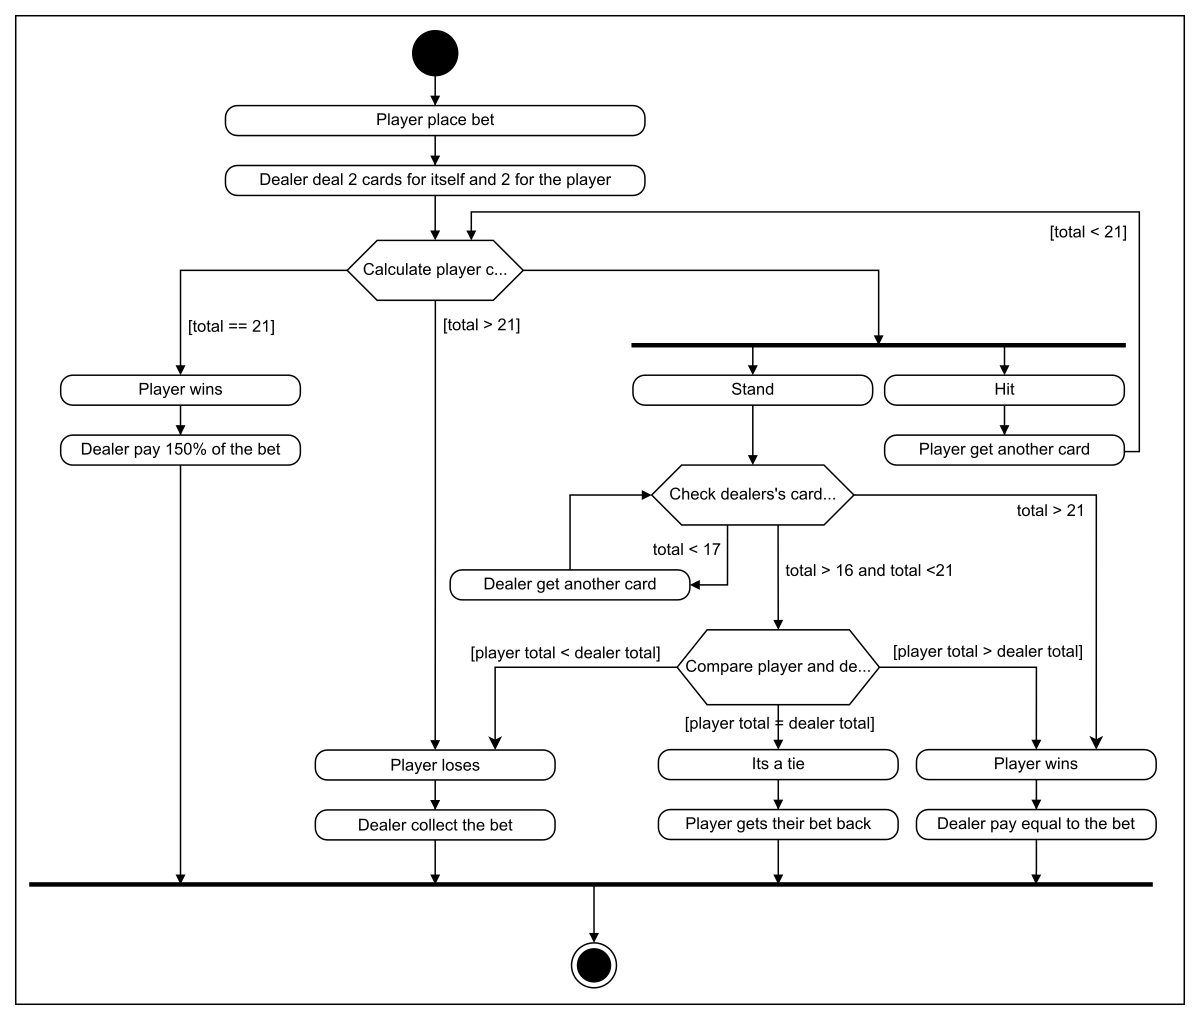
\includegraphics[width=0.5\textwidth]{Images/chapter_12/section_6271264281067520/6297873330077696.png}
 \caption{The activity diagram for the Blackjack game play}
\end{figure}

We've looked at the activity diagrams of the Blackjack game. In the next lesson, we will present the code for our designed classes in some of the most popular languages.

% End of section content